\begin{figure}[h!]
	\centering
	
	
	\tikzset{every picture/.style={line width=0.75pt}} %set default line width to 0.75pt        
	
	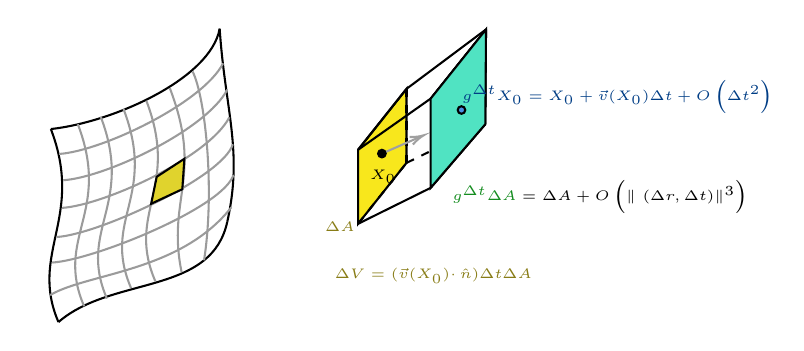
\begin{tikzpicture}[x=0.75pt,y=0.75pt,yscale=-1,xscale=1]
		%uncomment if require: \path (0,300); %set diagram left start at 0, and has height of 300
		
		%Shape: Polygon [id:ds09456144699087154] 
		\draw  [fill={rgb, 255:red, 248; green, 231; blue, 28 }  ,fill opacity=1 ] (178.67,88.67) -- (202,59.33) -- (202,95) -- (178.67,124.33) -- cycle ;
		%Curve Lines [id:da4604489904212945] 
		\draw    (30.67,78.67) .. controls (61,75.33) and (107.67,54.33) .. (112,30.33) ;
		%Curve Lines [id:da6967720169789406] 
		\draw    (34.33,171.67) .. controls (20,138.33) and (47,121.33) .. (30.67,78.67) ;
		%Curve Lines [id:da35266638580627574] 
		\draw    (34.33,171.67) .. controls (54,154.56) and (86.77,156.23) .. (104.47,141.91) .. controls (109.87,137.54) and (113.87,131.68) .. (115.67,123.33) ;
		%Curve Lines [id:da4240338947405422] 
		\draw    (115.67,123.33) .. controls (123.33,89) and (114.67,70) .. (112,30.33) ;
		%Curve Lines [id:da691890187484379] 
		\draw [color={rgb, 255:red, 155; green, 155; blue, 155 }  ,draw opacity=1 ]   (46.67,164) .. controls (32.33,130.67) and (60,119) .. (43.67,76.33) ;
		%Curve Lines [id:da4043207998593765] 
		\draw [color={rgb, 255:red, 155; green, 155; blue, 155 }  ,draw opacity=1 ]   (57.67,160.33) .. controls (43.33,127) and (71,115.33) .. (54.67,72.67) ;
		%Curve Lines [id:da5252238052351152] 
		\draw [color={rgb, 255:red, 155; green, 155; blue, 155 }  ,draw opacity=1 ]   (69.33,155.33) .. controls (55,122) and (82,111.67) .. (65.67,69) ;
		%Curve Lines [id:da31270908120152363] 
		\draw [color={rgb, 255:red, 155; green, 155; blue, 155 }  ,draw opacity=1 ]   (81,152) .. controls (66.67,118.67) and (93,107.67) .. (76.67,65) ;
		%Curve Lines [id:da6303057039241056] 
		\draw [color={rgb, 255:red, 155; green, 155; blue, 155 }  ,draw opacity=1 ]   (93.67,147.67) .. controls (86.33,112) and (104.33,101.67) .. (88,59) ;
		%Curve Lines [id:da8218053838878148] 
		\draw [color={rgb, 255:red, 155; green, 155; blue, 155 }  ,draw opacity=1 ]   (104.47,141.91) .. controls (109.67,109) and (105.33,64) .. (99,51) ;
		%Curve Lines [id:da8308238051916903] 
		\draw [color={rgb, 255:red, 155; green, 155; blue, 155 }  ,draw opacity=1 ]   (113.67,47) .. controls (103.67,66.33) and (55,89.33) .. (34.67,90.67) ;
		%Curve Lines [id:da02053447085552529] 
		\draw [color={rgb, 255:red, 155; green, 155; blue, 155 }  ,draw opacity=1 ]   (115.67,59.67) .. controls (105.67,79) and (57,102) .. (36.67,103.33) ;
		%Curve Lines [id:da5282822241031992] 
		\draw [color={rgb, 255:red, 155; green, 155; blue, 155 }  ,draw opacity=1 ]   (116.67,73) .. controls (106.67,92.33) and (56.33,115.33) .. (36,116.67) ;
		%Curve Lines [id:da23816183015057169] 
		\draw [color={rgb, 255:red, 155; green, 155; blue, 155 }  ,draw opacity=1 ]   (118.33,86) .. controls (113.67,101.67) and (54,129.33) .. (33.67,130.67) ;
		%Curve Lines [id:da569405412784046] 
		\draw [color={rgb, 255:red, 155; green, 155; blue, 155 }  ,draw opacity=1 ]   (118.67,100.67) .. controls (114,116.33) and (51.67,141.67) .. (31.33,143) ;
		%Curve Lines [id:da11295701912713185] 
		\draw [color={rgb, 255:red, 155; green, 155; blue, 155 }  ,draw opacity=1 ]   (117.67,116.33) .. controls (93,147.67) and (48.33,148) .. (30.33,158.67) ;
		%Straight Lines [id:da4575502778776137] 
		\draw    (178.67,88.67) -- (202,59.33) ;
		%Straight Lines [id:da09259804747392031] 
		\draw    (178.67,124.33) -- (178.67,88.67) ;
		%Straight Lines [id:da5208713033396146] 
		\draw  [dash pattern={on 3pt off 3pt}]  (202,95) -- (202,59.33) ;
		%Straight Lines [id:da5610562629835913] 
		\draw  [dash pattern={on 3pt off 3pt}]  (178.67,124.33) -- (202,95) ;
		%Straight Lines [id:da25649545572729315] 
		\draw [color={rgb, 255:red, 160; green, 160; blue, 160 }  ,draw opacity=1 ][line width=0.75]    (190.17,90.5) -- (208.5,82.47) ;
		\draw [shift={(210.33,81.67)}, rotate = 156.35] [color={rgb, 255:red, 160; green, 160; blue, 160 }  ,draw opacity=1 ][line width=0.75]    (6.56,-1.97) .. controls (4.17,-0.84) and (1.99,-0.18) .. (0,0) .. controls (1.99,0.18) and (4.17,0.84) .. (6.56,1.97)   ;
		%Shape: Circle [id:dp4347516737268753] 
		\draw  [fill={rgb, 255:red, 0; green, 0; blue, 0 }  ,fill opacity=1 ] (188.33,90.5) .. controls (188.33,89.49) and (189.15,88.67) .. (190.17,88.67) .. controls (191.18,88.67) and (192,89.49) .. (192,90.5) .. controls (192,91.51) and (191.18,92.33) .. (190.17,92.33) .. controls (189.15,92.33) and (188.33,91.51) .. (188.33,90.5) -- cycle ;
		%Straight Lines [id:da9970436041671149] 
		\draw    (213.67,64) -- (240.33,30.67) ;
		%Straight Lines [id:da342511901706108] 
		\draw    (213.67,107) -- (213.67,64) ;
		%Straight Lines [id:da5902552900557785] 
		\draw    (240,76.33) -- (240.33,30.67) ;
		%Straight Lines [id:da8931061197488246] 
		\draw    (213.67,107) -- (240,76.33) ;
		%Straight Lines [id:da6468976920553455] 
		\draw    (178.67,124.33) -- (213.67,107) ;
		%Straight Lines [id:da7362591464280432] 
		\draw    (178.67,88.67) -- (213.67,64) ;
		%Straight Lines [id:da5565256227844282] 
		\draw    (202,59.33) -- (240.33,30.67) ;
		%Straight Lines [id:da34026137798256473] 
		\draw  [dash pattern={on 3pt off 3pt}]  (202,95) -- (240,76.33) ;
		%Shape: Polygon [id:ds9396511578559401] 
		\draw  [fill={rgb, 255:red, 80; green, 227; blue, 194 }  ,fill opacity=1 ] (240.33,30.67) -- (240,76.33) -- (235.75,81.28) -- (213.67,107) -- (213.67,64) -- cycle ;
		%Shape: Circle [id:dp5366643183971873] 
		\draw  [fill={rgb, 255:red, 74; green, 144; blue, 226 }  ,fill opacity=1 ] (226.67,69.5) .. controls (226.67,68.49) and (227.49,67.67) .. (228.5,67.67) .. controls (229.51,67.67) and (230.33,68.49) .. (230.33,69.5) .. controls (230.33,70.51) and (229.51,71.33) .. (228.5,71.33) .. controls (227.49,71.33) and (226.67,70.51) .. (226.67,69.5) -- cycle ;
		%Shape: Polygon [id:ds3478569100900799] 
		\draw  [fill={rgb, 255:red, 224; green, 211; blue, 45 }  ,fill opacity=1 ] (95,93) -- (94,107.67) -- (79,114.67) -- (81.67,101.67) -- cycle ;
		
		% Text Node
		\draw (183,96.73) node [anchor=north west][inner sep=0.75pt]  [font=\tiny]  {$X_{0}$};
		% Text Node
		\draw (227.33,53.73) node [anchor=north west][inner sep=0.75pt]  [font=\tiny,color={rgb, 255:red, 0; green, 61; blue, 133 }  ,opacity=1 ]  {$g^{\Delta t} X_{0} =X_{0} +\vec{v}( X_{0}) \Delta t+O\left( \Delta t^{2}\right)$};
		% Text Node
		\draw (161.33,122.07) node [anchor=north west][inner sep=0.75pt]  [font=\tiny,color={rgb, 255:red, 136; green, 124; blue, 22 }  ,opacity=1 ]  {$\Delta A$};
		% Text Node
		\draw (222.67,102.07) node [anchor=north west][inner sep=0.75pt]  [font=\tiny]  {$\textcolor[rgb]{0.08,0.55,0.12}{g^{\Delta t} \Delta A} =\Delta A+O\left( \| \ ( \Delta r,\Delta t) \| ^{3}\right)$};
		% Text Node
		\draw (166,144.4) node [anchor=north west][inner sep=0.75pt]  [font=\tiny,color={rgb, 255:red, 136; green, 124; blue, 22 }  ,opacity=1 ]  {$\Delta V=(\vec{v}( X_{0}) \cdotp \hat{n}) \Delta t\Delta A$};
		
		
	\end{tikzpicture}
\end{figure}